\section{Lecture 8: 02/24/21}

\begin{question}
True or false: If $(G, *)$ is a group, then $a * b = b * a$ for all $a, b \in G$.
\end{question}

This is false! This is not in the group axioms, and is not necessarily true.

\begin{definition}[Abelian]
A group $(G, *)$ is \textit{abelian} or \textit{commutative} if $a*b=b*a$ for all $a,b\in G$.
\end{definition}

\subsection{Examples of Groups}

\begin{example}
Here are some examples of groups:
\begin{itemize}
    \item $(\Z, +)$
    \item $(\R, +)$
    \item $(\Q, +)$
    \item $(\Q\setminus \{0\}, \cdot)$
    \item $(U_n, \cdot_n)$
    \item $(\Z_n, +_n)$
    \item $(\text{permutations on }S, \cdot)$, also denoted by $(S_n, \circ)$.
\end{itemize}
Note that almost all of these are abelian, except the last one which is non-abelian when $n > 2$.
\end{example}

\subsection{Subgroups}

\begin{definition}[Subgroup]
A \textit{subgroup} of a group $(G, *)$ is a subset $H$ of $G$ such that $(H, *)$ is a group.
\end{definition}

\begin{example}
$\Z$ is a subgroup of $(\R, +)$.
\end{example}

Let's think of general simple cases. Let $(G, *)$ be a group. What are some subgroups of $G$?
\begin{itemize}
    \item $\{e\}$ is a subgroup (the ``trivial subgroup'').
    \item $G$ is a subgroup (the ``improper subgroup'').
\end{itemize}

\begin{example}[Subgroups of $(\Z_6, +)$]
\quad
\begin{itemize}
    \item The smallest subgroup of $(\Z_6, +_6)$ including $2$ is $\{0, 2, 4\}$ (We denote the subgroup by $\langle 2 \rangle$.) 
\end{itemize}
\end{example}

\begin{example}[TopSpin!]
One sentence explanation: you can rotate numbers in the purple and rotate the entire thing. There are 20 slots where the numbers can go, and we'll number these slots as shown the left picture.

\begin{figure}[h]
    \centering
    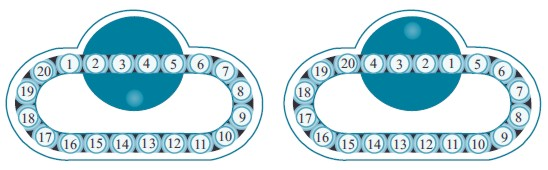
\includegraphics[width=0.5\textwidth]{notes/images/topspin.jpg}
    \caption{TopSpin}
    \label{fig:topspin}
\end{figure}

We can describe any move by saying what it does to the slots. For example, if you rotate the blue dial, that swaps the numbers in slots $1$ and $4$, as well as the numbers in slots $2$ and $3$. We would describe this as $(1 \ 4)(2 \ 3)$ in cycle notation. Rotating the entire thing clockwise can be described as $(1 \ 2 \ 3 \dots \ 20)$. Why is this a group?

\begin{itemize}
    \item Closure: If $M_1, M_2 \in T$, then $M_1 \circ M_2 \in T$ because $M_1 \circ M_2$ is a move.
    \item Identity: ``Do nothing" is the identity, $e \circ M = M \circ e = M$.
    \item Inverses: Every move can be undone.
    \item Associativity: Note that $T$ is a subset of $S_{20}$ (i.e. if $M_1, M_2, M_3 \in T$, then $M_1, M_2, M_3 \in S_{20}$). Since $S_{20}$ is a group, $M_1 \circ (M_2 \circ M_3) = (M_1 \circ M_2) \circ M_3$.
\end{itemize}

\end{example}

\subsection{The Subgroup Criterion}

\begin{proposition}[The Subgroup Criterion]
Let $(G, *)$ be a group. A nonempty subset $H$ of $G$ is a subgroup of $G$ iff, for every $a, b \in H$, we have $a * b^{-1} \in H$.
\end{proposition}

\begin{proof}
$(\implies)$. Apply the inverses property, so $b^{-1}$ is in $H$, and then apply closure, so $a * b^{-1}$ is in $H$. 

$(\impliedby)$. We want to show that $H$ is a group, so we show the four axioms:
\begin{itemize}
    \item Identity: Let $a \in H$ (which is possible since $H$ is nonempty). Then, $a * a^{-1} \in H$ by the hypothesis.
    \item Let $a \in H$. We just showed that $e \in H$, so $e * a^{-1} \in H$ by hypothesis.
    \item Closure: Let $a, b \in H$. We just showed that $b^{-1} \in H$, so $a * (b^{-1})^{-1} = a * b \in H$.
    \item Associativity is inherited from $G$.
\end{itemize}
\end{proof}

We can write a shorter proof that $T$ is a group by showing it is a subgroup of $S_{20}$ via the Subgroup Criterion (done in class, exercise for the reader).